\section{Using Veritracer}

During the first public presentation, J.M. Muller asked us if our tool could handle the following case illustrated in his book:

 \begin{equation}
   u_{n} = 111 - \dfrac{1130}{u_{n-1}} + \dfrac{3000}{u_{n-1}u_{n-2}}
   \label{eq:muller_sequence_un}
 \end{equation}

The fixed points of this sequence are the roots of the polynomial:

\quad $u^3 - 111u^2 + 1130u - 3000 = (u-5)(u-6)(u-100)$

With the chosen initial values, $u_0=2$ and $u_1=-4$, the mathematical answer is 6.

\subsection{Running the code with Veritracer}

We will first reproduce the experiment of D. Stott Parker~\cite{parker1997monte}.

\begin{question}
    \begin{enumerate}[(a)]
\item Compile and test {\tt muller.c}
\item Modify {\tt Makefile} to compile with {\tt verificarlo}
\item Collect 32 results with virtual precision 53.
\item Compute the number of significant digits $s$.

$\Rightarrow$ As you can see the program is converging to the dominant root of the polynomial {\it i.e.} 100, with maximum precision! Therefore, by looking only to the final precision one could conclude that this is the correct answer\\~\\

\end{enumerate}
\end{question}

We will now do the experiment with veritracer to better understand this result.

\begin{question}
    \begin{enumerate}
        \item Type the command {\tt verificarlo -{}-help} to print how to call veritracer usage
        \item Type the command, and check the output and the {\tt .map} generated files \newline
        {\tt verificarlo -{}-verbose -{}-tracer muller.c -o muller -{}-function muller1 }
        \item Remove the current location map and launch veritracer in backtrace mode with the following command: {\tt verificarlo -{}-verbose -{}-tracer muller.c -o muller -{}-function muller1  -{}-tracer-backtrace}
        \item Run the program in the tracer environment with the following command: \newline
        {\tt veritracer launch -{}-force -{}-binary muller -{}-jobs 29}
        \item Check the content of the {\tt .vtrace} directory
        \item To launch the trace analysis run the command: {\tt veritracer analyze } and check the result in  the file {\tt .vtrace/veritracer.000bt}
        \item Plot the result with the provided {\it ad-hoc} script with the following command: \newline
        {\tt veritracer plot .vtrace/veritracer.000bt}
        \item It is possible to add invocation information with the following command: \newline
        {\tt veritracer plot .vtrace/veritracer.000bt -{}-invocation-mode}
        \item and basic statistics: {\tt veritracer plot .vtrace/veritracer.000bt -{}-invocation-mode -{}-mean -{}-std}
%rm locationInfo.map
%verificarlo -{}-verbose -{}-tracer muller.c -o muller -{}-function muller1  -O3
%locationInfo.map -> vide Why ?

%verificarlo -{}-verbose -{}-tracer muller.c -o muller -{}-function muller1  -O3
%verificarlo -{}-verbose -{}-tracer muller.c -o muller -{}-function muller1
%-{}-tracer-backtrace -O3 -{}-tracer-level temporary
%cat locationInfo.map


%veritracer launch -{}-force -{}-binary muller -j 29
%veritracer analyze
%empty traces ? Pourquoi


%verificarlo -{}-verbose -{}-tracer muller.c -o muller  -{}-tracer-backtrace
%-O3 -{}-tracer-level temporary
    \end{enumerate}
    $\Rightarrow$ NEW update: a pre-release GUI to plot and navigate in the trace is available on github for a more friendly user experience
\end{question}

$\Rightarrow$ Figure~\ref{fig:muller_sequence_un} has been automatically generated thanks to veritracer. It shows the evolution of the significant digits with the iteration. We can observe a gradual degradation of the precision until it reaches no significant digits. Then the precision is gradually improving to reach the maximum attainable in double precision format, {\it i.e.} 17. This plot allow us to conclude that the generated results, while being precise, as lost all its accuracy.

For the final experiment of this section we will use veritracer on the Tchebychev polynomial from this tutorial.

\begin{question}
  \begin{enumerate}[(a)]
      \item Experiment veritracer on the Tchebychev Polynomial evaluation between $0$ and $1$ by $0.001$.
      $\Rightarrow$ The result is presented in figure~\ref{fig:veritcheby}.

%rm locationInfo.map
%verificarlo -{}-tracer tchebychev.c -o tchebychev -O3  -{}-tracer-level
%temporary -{}-tracer-backtrace
%cat locationInfo.map

%veritracer launch -{}-force -{}-binary "./tchebychev FACTORED 100" -j 29 &&
%veritracer analyze

%veritracer plot .vtrace/veritracer.000bt -{}-invocation-mode -{}-mean -{}-std
%
%cat locationInfo.map |grep factored| grep ret
%veritracer plot .vtrace/veritracer.000bt -{}-invocation-mode -{}-mean -{}-std
%-v $$

%cat locationInfo.map |grep horner| grep ret
%veritracer launch -{}-force -{}-binary "./tchebychev  HORNER 100" -j 29 &&
%veritracer analyze
%veritracer plot .vtrace/veritracer.000bt -{}-invocation-mode -{}-mean -{}-std
%-v $$

  \end{enumerate}
\end{question}

 \begin{figure}[h!]
  \centering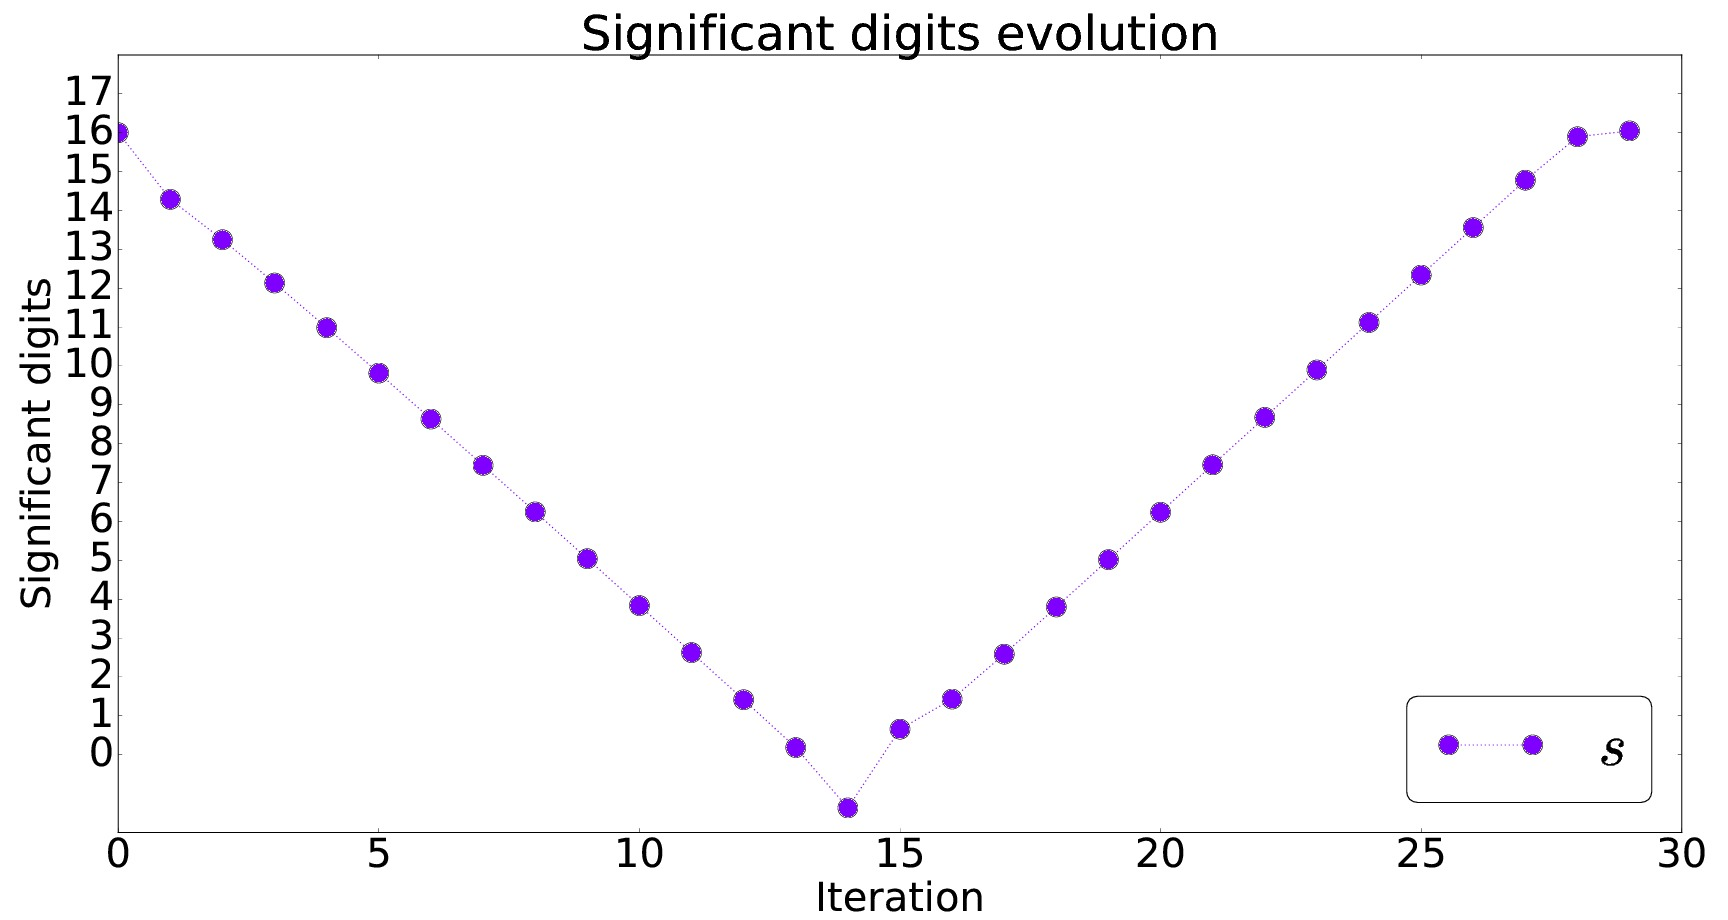
\includegraphics[width=0.8\linewidth]{muller_sequence_un.jpg}
  \caption{The evolution of the number of significant decimal digits ($s$) over time
     for the sequence $u_n$ in equation~\ref{eq:muller_sequence_un}.
    For $n=14$, $s$ is below 0 means that $u_{14}$ has no correct decimal digits.
     Only checking the final results is not enough to detect accuracy loss.
  }

 \label{fig:muller_sequence_un}
 \end{figure}
%
%
\begin{figure}[h!]
  \centering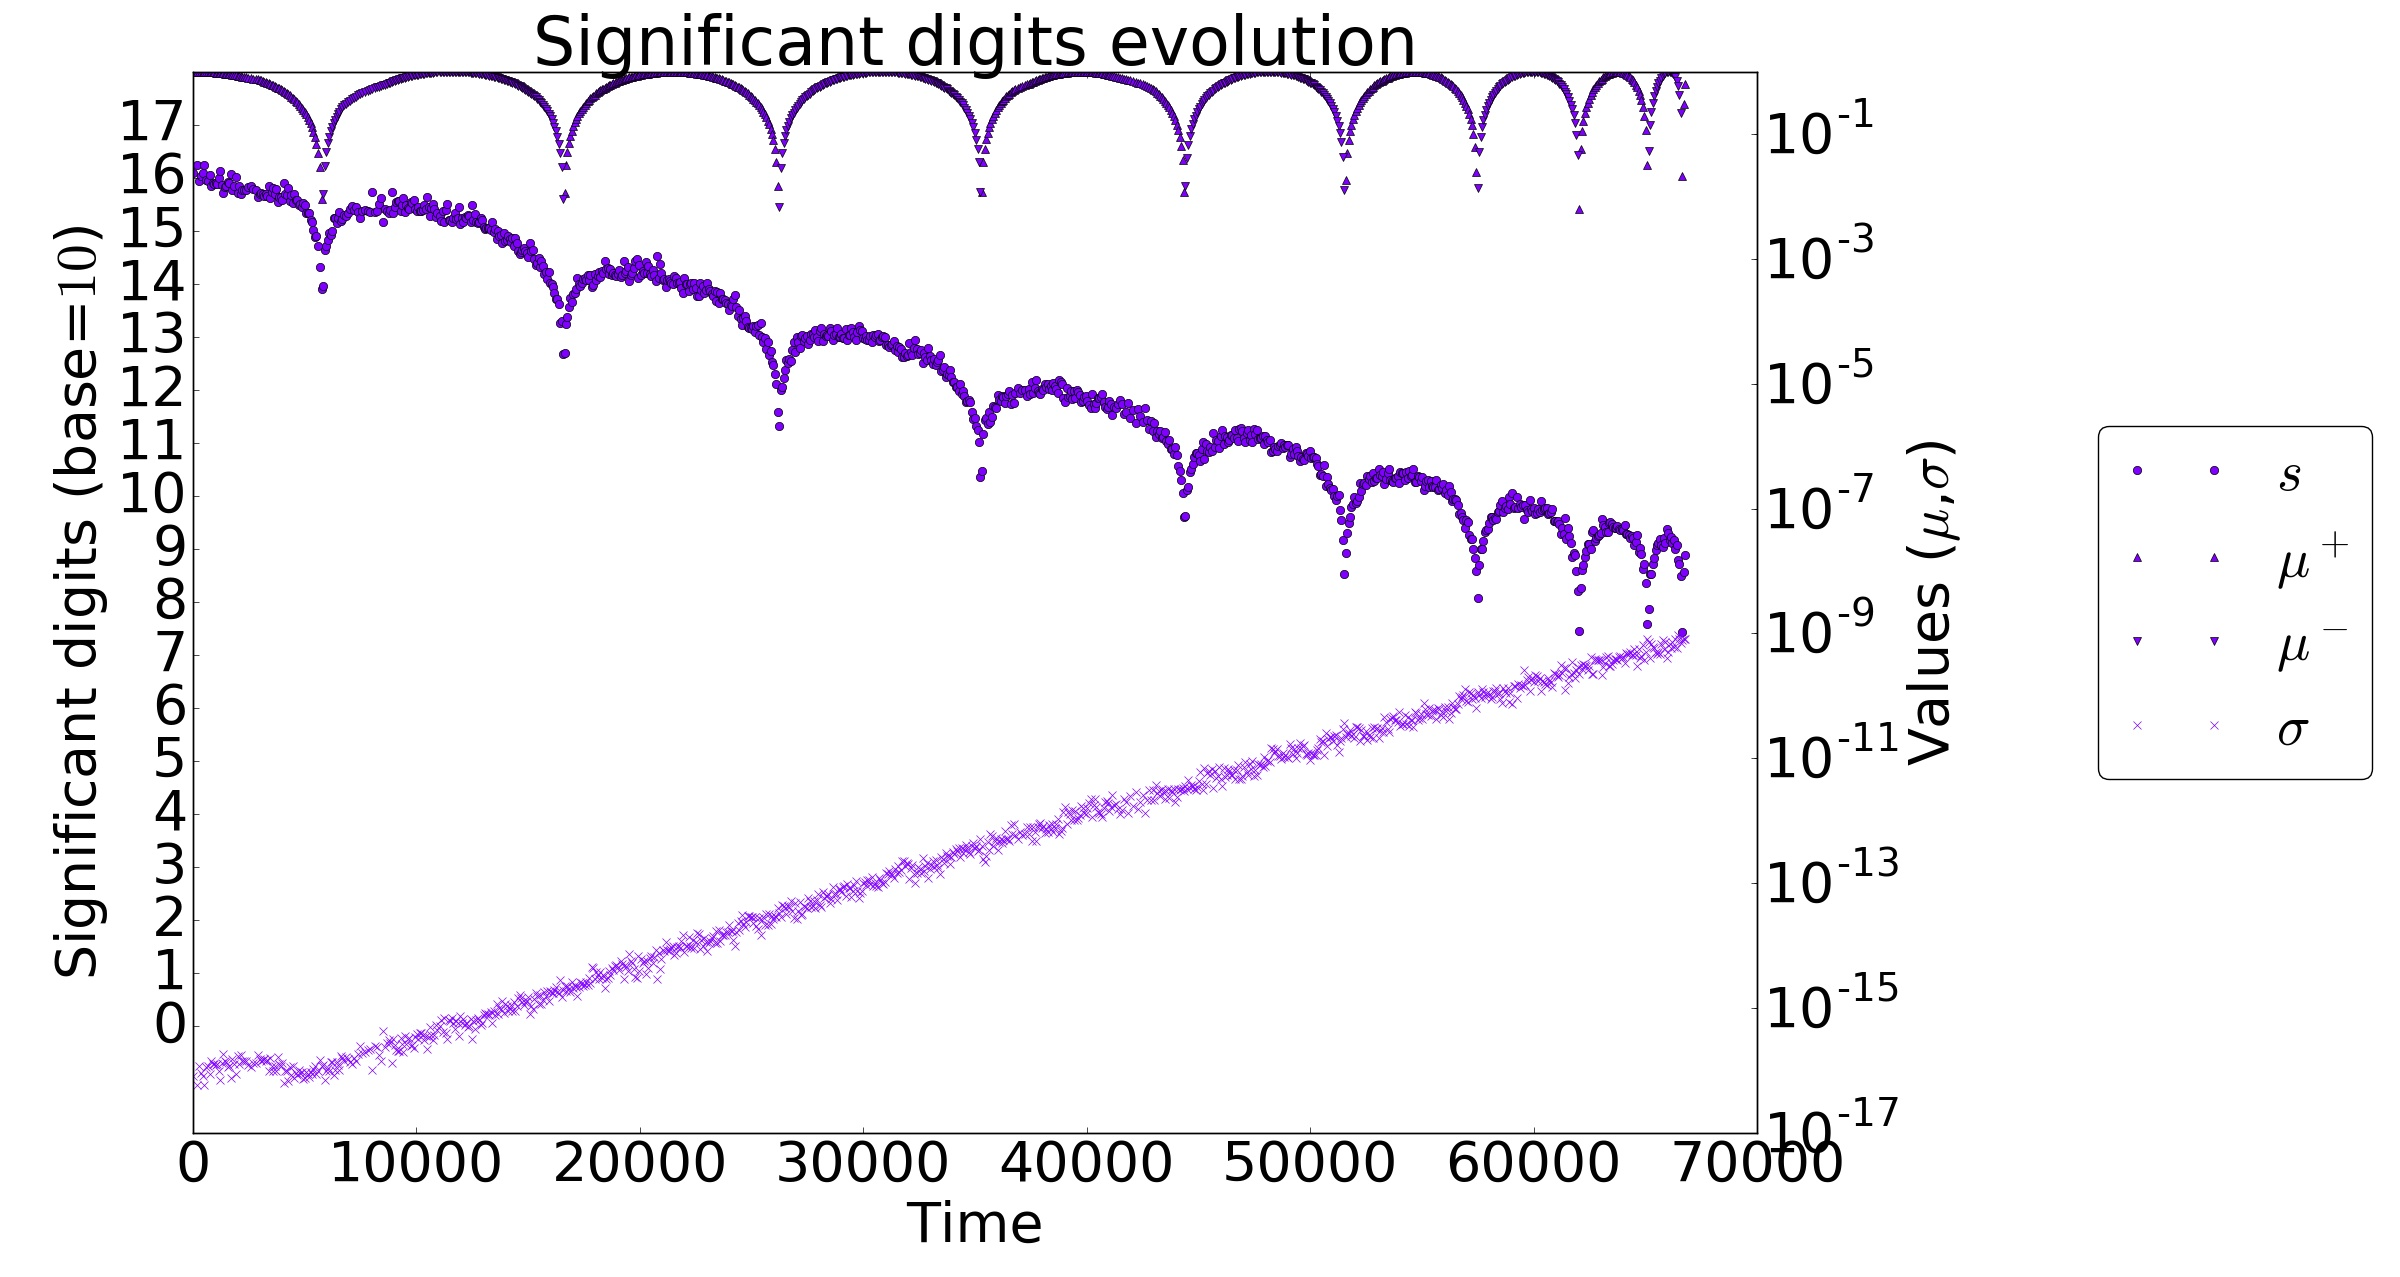
\includegraphics[width=1\linewidth]{tcheby_veritracer_large_font.jpg}
 \caption{The evolution of the number of significant decimal digits ($s$) over time
     for the evaluation of the tchebytchev polynomial used in this tutorial, from $0$ to $1$ by $0.001$.
  }
 \label{fig:veritcheby}
 \end{figure}
%
%
 ~\\~\\$\Rightarrow$ Veritracer contextualizes and traces variable precision over time: it helps to understand the arithmetic behavior of a program. It allows to focus program analysis on a limited set of functions, variables and inputs context.
%
%\FloatBarrier
%\clearpage

